\chapter{Building Envelope Form Generation and Thermal Optimisation}

\section{Methodology of Thermal Optimisation and Form Generation}

The information presented so far requires at this point that a clear methodology, properly sequenced, and categorised, formulated out of the concepts and tools illustrated so far in the thesis.

To recapitulate the purpose of the thesis; the aim is to provide a practical method, sufficiently supported by previous experimentation, of designing a building envelope which meets the thermal performance criteria of the designer, through iterative environmental simulation and algorithmic optimisation, algorithmic form generation and regeneration.

The proposed procedure to guide such and endeavour, is based on the elements of the process described in the previous chapters, but differs in sequence to suite the natural order of the design process, and it is as follows:

\begin{enumerate}
	\item Analysis of envelope form
	\item Determination of thermal criteria
	\item Selection of suitable digital simulation and modelling environment
	\item Selection of suitable form generation and/or optimisation algorithms
\end{enumerate}

\paragraph{Introduction of Algorithmic Input to Design Process} \mbox{}\\

An important issue to be considered is the point at which algorithm is introduced to the design process. The introduction of algorithm (and simulation for that matter) at a very early stage as opposed to at a point when the schematic design has been almost finished would greatly influence the final product; as the former is considered pure form generation governed by optimisation algorithms, while the latter is considered optimisation of a geometry which has already been defined by the architect, and in turn defining the major optimisable variables.

Although the above would suggest that algorithmic form generation is best introduced at the earliest stage possible, this is not practical as it would mean that endless possibilities can be explored with no regard to user requirements. Therefore, for the sake of simplicity and practicality, it has been assumed that a conceptual form has been designed and used as a basis for further algorithmic optimisation. Form generation in this case is mostly \emph{regeneration} of the modelled geometry representing the building envelope.

\paragraph{Multi-criterion Optimisation} \mbox{}\\

Many of the cases presented in chapter 4 have showcased optimisation of envelopes with regard to only one variable; i.e. single-criterion optimisation (albeit with the exceptions of sections such as \ref{sec:KendallPavilion}), which was for the sake of making a clear and simple illustration of one concept or another. However, thermal optimisation in real world will almost always demand optimisation with more than one variable taken into consideration.

New problems will present themselves when shifting from single to multiple criterion optimisation, but by far the most important and influential is the problem of \emph{variable weighting system}, which is essentially the importance of each variable (external shading, fenestration\ldots etc.) in relation to the other variables. This should be studied and planned carefully by the architect, as conflicting variables will often demand very different solutions for each to be at optimum performance, and therefore the effect of each on the overall performance should be studied by the architect, possibly with the support of modelling and environmental simulation programs.

Another solution which in some cases might be practical, is to create reference points within the architectural space from which to measure the overall performance of the building envelope regardless of each variable and be used as the driving force behind the optimisation algorithm.

\subsection{Analysis and Categorisation of Envelope Form}

As described earlier (see page \pageref{BuildEnvDef}), any building envelope is composed of the architectural physical elements that separate the inside from the outside, creating an \emph{envelope} or emph{enclosure} for the building.

Although this definition applies to almost all building envelopes, they would vary greatly from one building to another, making the task at hand; which is the utilisation of algorithmic design and thermal simulation to achieve thermally eficient buildings, inefficient or even practically meaningless, unless proper categorisation of building envelope design is made.

This is due to the fact that with differences between building enclosure designs, the variables that affect the thermal performance of the envelope will have varying degrees of impact, sometimes even reaching almost zero impact in some cases; having mentioned above the importance of weighting in multi-criterion optimisation, this would especially important to determine which variable should be given the priority over others.

\paragraph{\emph{Phylogenesis} and the Categorisation of Building Envelopes}\mbox{}

One interesting way of categorising building enclosures, is the endevour undertaken by the \emph{Foreign Office Architects} to categorise their own work in a book named \emph{Phylogenesis: FOA's Ark} \cite{foa04}. The categorisation system resembles a biological evolutionary tree, that starts from one point and branches into different species through several evolutionary stages (figures \ref{fig:Phylogenesis} and \ref{fig:FOAEnvelopes}).

Regardless of the concept, the categorisation of building envelopes used by the Foreign Office Architects (FOA), makes an excellent working ground for analysis of different envelope forms, and defining the the thermal variables and their level of importance.

\begin{sidewaysfigure}[htbp]
	\centering
	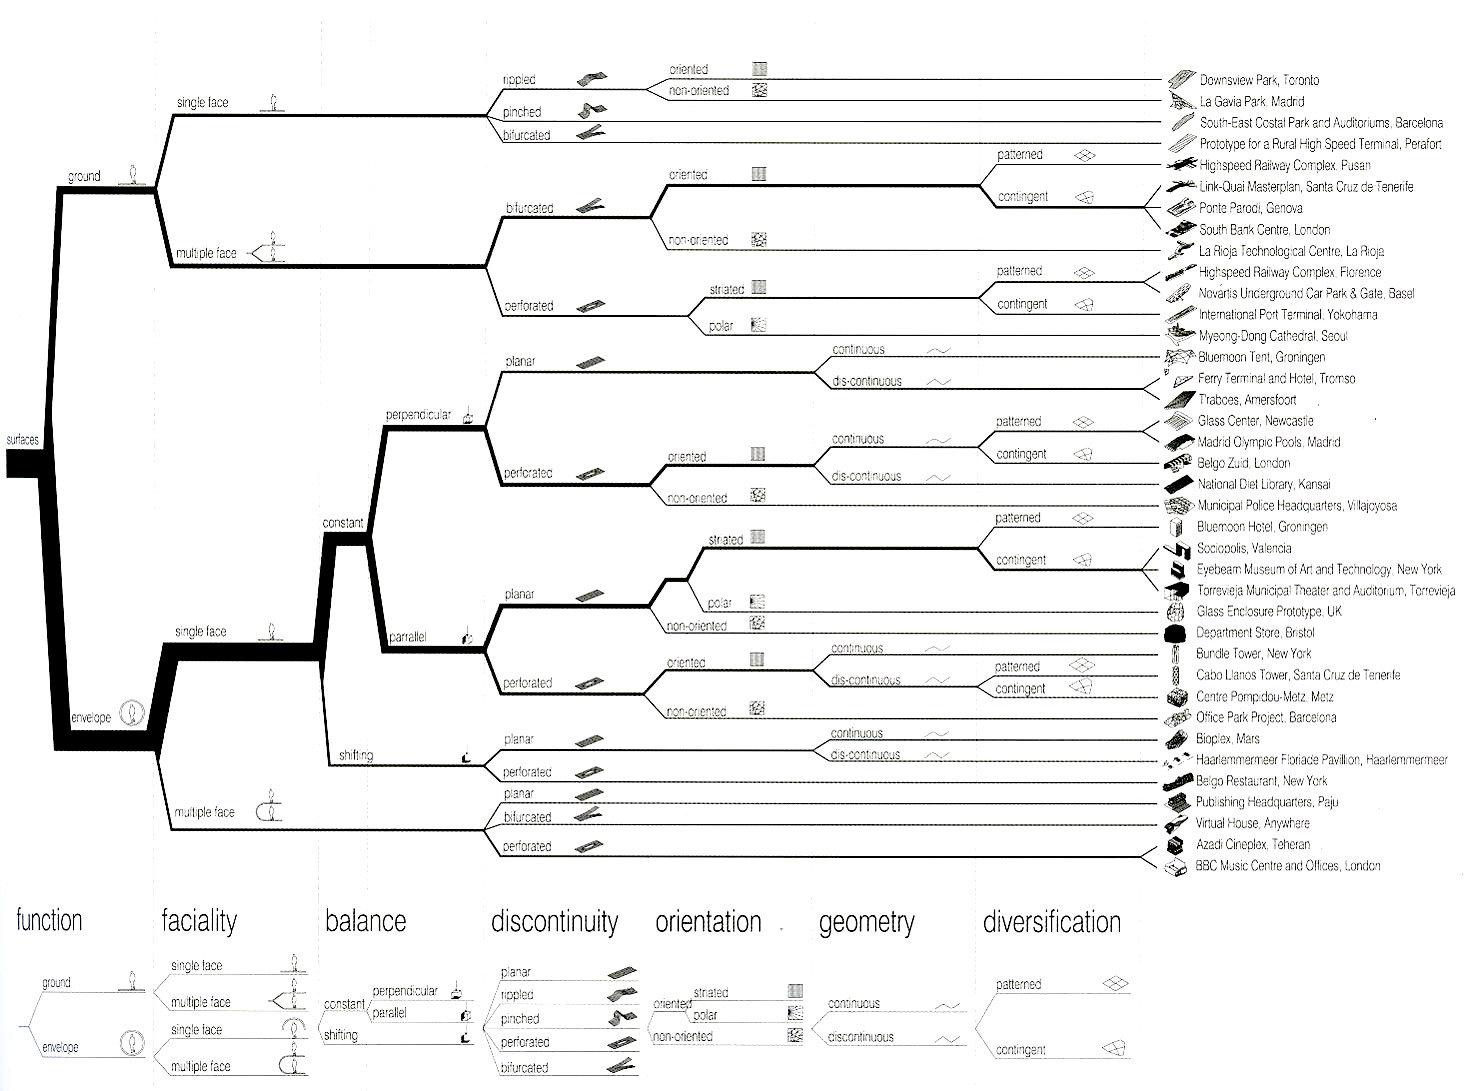
\includegraphics[width=20cm]{./Images/1-Phylogenesis}
	\caption[FOA Phylogenesis]{Sturcutres Categorisation of FOA Work, Including Envelope Categorisation According to \emph{Phylogenesis} \cite{foa04}}
	\label{fig:Phylogenesis}
\end{sidewaysfigure}

\begin{figure}[H]
	\centering
	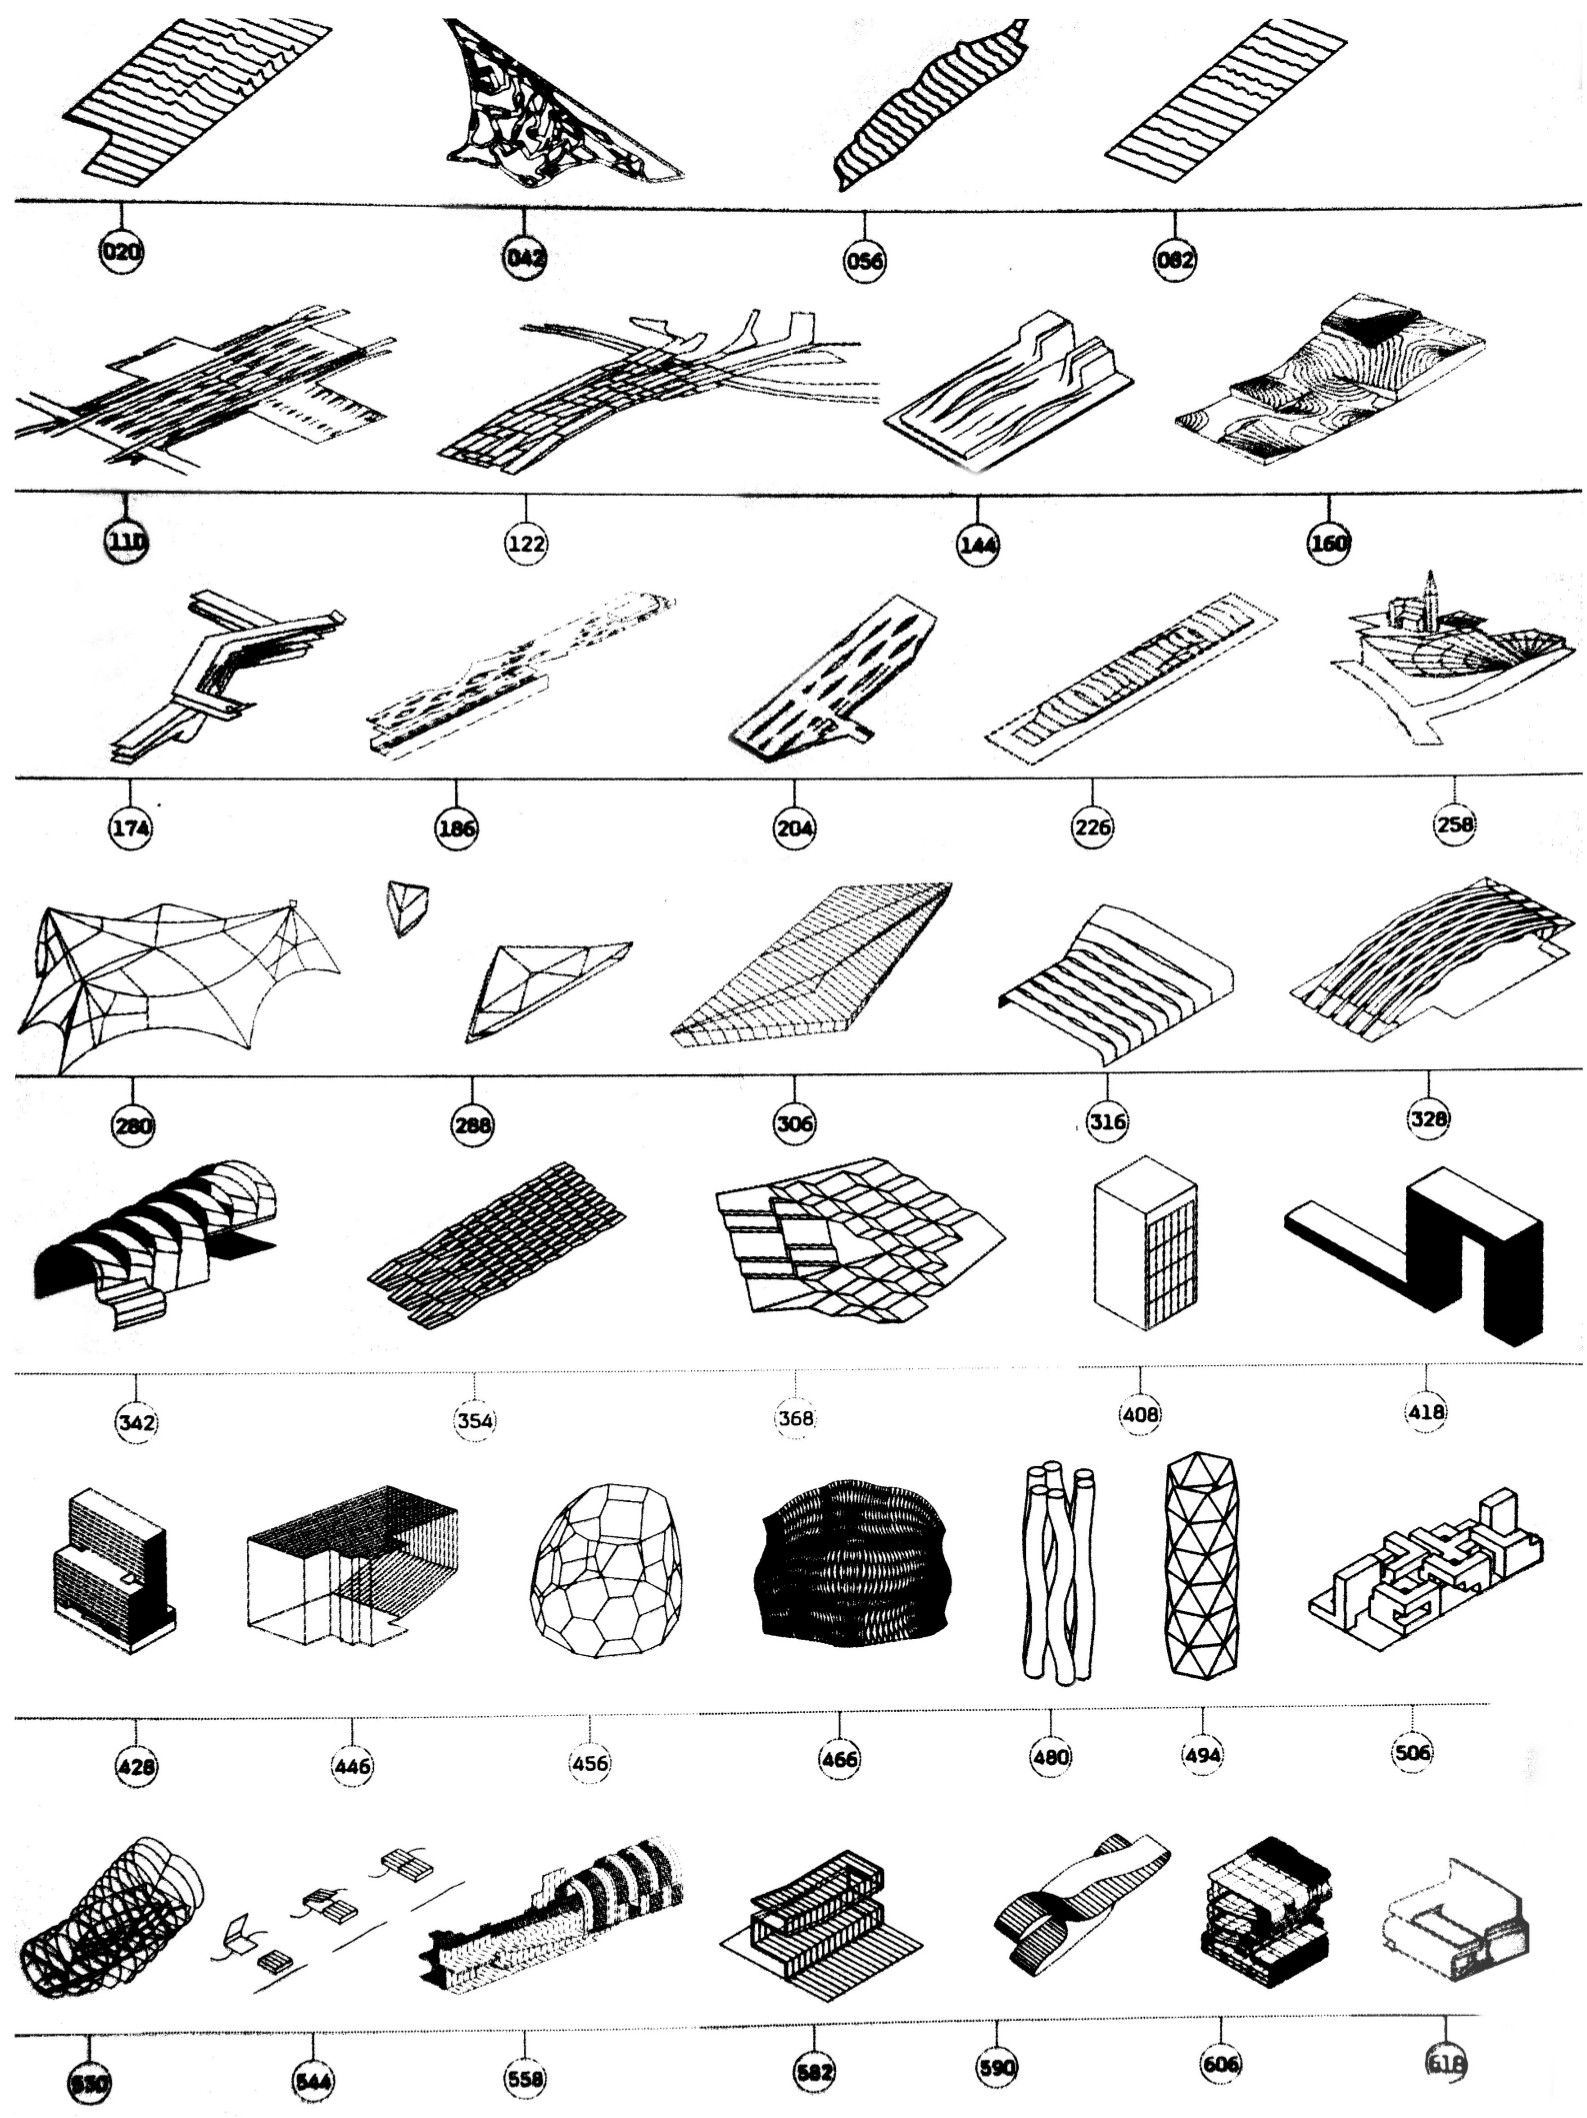
\includegraphics[width=\textwidth]{./Images/2-Envelopes}
	\caption[FOA Building Envelopes]{Examples of Structures and Building Envelopes by FOA \cite{foa04}}
	\label{fig:FOAEnvelopes}
\end{figure}


\subsection{Determination of Thermal Criteria}

Having created a system of categorisation in which any envelope form can mostly fit under a category; the thermal design through algorithm and simulation should be guided by the variables that affect the particular envelope form the most.

Here we refer to the design variables listed earlier in Chapter 3 (see page \pageref{sec:ThermalDesignVariables}), which are concerned with thermal design through passive solar control. This holds true even in chapter 4, and has been done with the intention to simplify the process and narrow the scope for easier understading throughout the thesis.

For the sake of convinience, the variables are relisted here in table form.

\begin{table}[H]
	\centering
	\begin{tabular}{l|l}
		\textbf{Shape}		&Surface-to-Volume Ratio\\
					&Orientation\\
					&\\
		\textbf{Fabric} 	&Shading\\
					&Surface Material Properties\\
					&\\
		\textbf{Fenestration}	&Size, Position and Orientation\\
					&Glazing Material\\
					&Closing Mechanism\\
					&External Shading\\
	\end{tabular}
	\caption{Thermal Design Variables}
	\label{tab:ThermalDesignVariables}
\end{table}

\subsubsection{Building Envelope Form and Variables}

Before proceeding with assigning variables as driving parameters in the algorithmic design process, the above stated variables must be further explained with illustrative examples (it is advised to refer to the material presented in Chapter 3, as this section is concerned only with the practical aspect of analysing building envelopes in terms of thermal design variables).

\paragraph{Surface-to-Volume Ratio}\mbox{}

The surface-to-volume ratio of any building is mainly affected by three factors:

\begin{enumerate}
	\item Envelope Geometry; such as square, dome, sphere, pyramid\ldots{}etc (figure .
	\item 
\end{enumerate}

\subsection{Selection of Simulation and Modelling Environment}

\textbf{``Here I will refer to the different simulation application shown in chapter 3, explaining that each program has strong and weak points, and that this is very important if the algorithm will be inputted directly into the simulation program using its scripting language}

\subsection{Selection of Form Generation and Optimisation Algorithms}

\textbf{``Here i will refer to the comparisons made in chapter 2 regarding the differences between different generative and performative algorithms, and which are more suitable for the kind of optimisation / form generation as per the selected envelope type''}


\section{Examples by Envelope Type}

\textbf{``This will be the section where i put each type of envelope and make a list of the applicable variables, simulation environments, and algorithms. This will be in the form of sketches of the envelope type and a schedule on the the other page with the suitable options''}

\section{Conclusions}
